\documentclass[10pt]{article}

% Math
\usepackage{amsmath,amsthm}
\usepackage{amssymb}
\usepackage{bm} % For better bold symbols

\usepackage{anysize}

% For better graphic
\usepackage{graphicx}
% Colors
% \definecolor{Blue}{rgb}{0.2,0.2,0.9}
% \definecolor{Green}{rgb}{0,0.6,0}
% \definecolor{Gray}{rgb}{0.5,0.5,0.5}
% \definecolor{Purple}{rgb}{0.58,0,0.82}
% \definecolor{background}{rgb}{0.98,0.98,0.95}

% For writing code
\usepackage{listings}
\lstdefinestyle{basicstyle}{
    backgroundcolor=\color{background},   
    commentstyle=\color{Green},
    keywordstyle=\color{Blue},
    numberstyle=\tiny\color{Gray},
    stringstyle=\color{Purple},
    basicstyle=\ttfamily\footnotesize,
    breakatwhitespace=false,         
    breaklines=true,                 
    captionpos=b,                    
    keepspaces=true,                 
    numbers=left,                    
    numbersep=5pt,                  
    showspaces=false,                
    showstringspaces=false,
    showtabs=false,                  
    tabsize=2
}
\lstset{style=basicstyle}

% Language settings
\usepackage[italian]{babel}

% Better tables
\usepackage{booktabs}

% Defining theorems
\usepackage{thmtools}

% References
\usepackage[italian]{cleveref}
\usepackage{nameref}

% Units of measure
\usepackage{siunitx}

% Better colors
\usepackage{xcolor}


% ============ MATH ============
% Vector bold
\newcommand{\ve}[1]{\bm{#1}}
% Tensor upright
\newcommand{\tens}[1]{\mathsf{#1}}
% Derivatives
\newcommand{\deriv}[3][]{
	\ensuremath{\frac{d^{#1}{#2}}{d{#3}^{#1}}}
}
\newcommand{\pderiv}[3][]{
	\ensuremath{\frac{\partial^{#1}{#2}}{\partial{#3}^{#1}}}
}
% Tale Che
\newcommand{\tc}{\ensuremath{\;\text{t.c.}\;}}
\newcommand{\tcq}{\ensuremath{\quad\text{t.c.}\quad}}
% Logic
\newcommand{\et}{\wedge}
\newcommand{\orr}{\vee}
\newcommand{\cond}{\mid}

% === Smashed ===
% Smashed hat
\newcommand{\shat}[1]{\vphantom{#1}\smash[t]{\hat{#1}}}

% === Operators ===
% Dominium
\DeclareMathOperator{\Dom}{Dom}
% Argmin & Argmax
\DeclareMathOperator*{\argmin}{argmin}
\DeclareMathOperator*{\argmax}{argmax}

% ------------ NEW THEOREMS ------------
% >> In Theorem Style
% Teorema
\newtheorem{theorem}{Teorema}[section]
\crefname{theorem}{Teorema}{Teoremi}
% >> In Definition Style
\theoremstyle{definition}
% Esempio
\newtheorem{example}{Esempio}[section]
\crefname{example}{Esempio}{Esempi}
% Proprietà
\newtheorem{property}{Proprietà}[subsection]
\crefname{property}{Proprietà}{Proprietà}
% Definizione
\newtheorem{definition}{Definizione}[section]
\crefname{definition}{Definizione}{Definizioni}
% Osservazione
\newtheorem{observation}{Osservazione}[subsection]
\crefname{observation}{Osservazione}{Osservazioni}

% ============ REFERENCES ============

% Named Cref
\newcommand{\Crefn}[1]{\Cref{#1} (\nameref{#1})}

% ============ TEXT ============
\newcommand{\im}[1]{\textsc{#1}}

%%% OPERATORS
    \DeclareMathOperator{\pr}{Pr}
\DeclareMathOperator{\erf}{erf}
\DeclareMathOperator{\Beta}{Beta}
\DeclareMathOperator{\Ga}{Ga}
\DeclareMathOperator{\Exp}{Exp}
\DeclareMathOperator{\Unif}{Unif}
\DeclareMathOperator{\Cov}{Cov}
\DeclareMathOperator{\corr}{corr}
\DeclareMathOperator{\NLL}{NLL}
\DeclareMathOperator{\bias}{bias}
%%%

%% MATH MISC
\newcommand{\HALF}{\frac{1}{2}}

%% PARENTESIS
\newcommand{\pare}[1]{
	\ensuremath{\left(#1\right)}
}
\newcommand{\spare}[1]{
	\ensuremath{\left[#1\right]}
}

%% TEXT IN MATH
\newcommand{\MLE}{\ensuremath{\text{MLE}}}

\begin{document}

\title{Note del corso\\\textsc{Machine Learning per la fisica applicata\\e fisica delle alte energie}}
\author{Raviola Alessio}
\date{\today}

\maketitle

%%%%%%%%%%%%%%%%%%%%%%%%%%%%%%%%%%%%%%%%%%%%%%%%%%%%%%%%%%%%%%%%%%%%%%%%
\section{Introduzione}
%
%
%%%%%%%%%%%%%%%%%%%%%%%%%%%%%%%%%%%%%%%%%%%%%%%%%%%%%%%%%%%%%%%%%%%%%%%%
\begin{quotation}
A computer program is said to learn from experience E with respecto to some
class of tasks T and performance measure P, if its performance at tasks in T, as
measured by P, improves with experience E.
\end{quotation}
L'impostazione del corso è di tipo \textit{probabilistico} (statistical
learning). Le quantità non note sono trattate come \textbf{variabili aleatorie}
(\im{random variables}) a cui viene associata una \textbf{distribuzione di
probabilità} (\im{probability distribution}) che descrive il set (pesato) di
valori che la variabile può assumere.

Abbiamo tre tipi di machine learning:
\begin{itemize}
\item \im{supervised learning};
\item \im{unsupervised learning};
\item \im{reinforcement learning};
\end{itemize}
il corso si focalizza sui primi due tipi.

\subsection{Supervised learning}
Il \textbf{compito} T consiste nell'imparare una mappa $f$ dagli input $x\in X$
agli output $y\in Y$. Gli \textbf{input} $x$ sono chiamati \im{features} (o
\im{covariates} o \im{predictors}) e sono in genere costituiti da un vettore
reale con dimensione fissata, ovvero abbiamo $X\equiv \mathbb{R}^D$. Gli
\textbf{output} sono chiamati \im{label} (o \im{target} o \im{response}).

L'\textbf{esperienza} E consiste in un \im{training set} $\mathcal{D}$ di $N$
coppie input-output:
\begin{equation}
\mathcal{D} = \left\{ (x_n, y_n) \right\}_{n=1}^N,
\end{equation}
dove \( N \) è detta \im{sample size}.

La \textbf{performance} dipenda dal compito T.

\subsubsection{Classificazione}
Problemi comuni in machine learning sono quelli di \textbf{classificazione}. In
un problema di questo tipo lo spazio degli output C è un set \textit{non
ordinato} di label \( y = \{ 1, 2, \ldots, C \} \) dette \im{classes}. Quello che
chiede il problema è di predire una classe dato un input, problemi di questo
tipo sono detti di \im{pattern recognition}\footnote{Se abbiamo solo due classi,
i.e. solo due output, allora il problema si dice di \im{classificazione
binaria}}.

\begin{example}[Classificazione specie di iris]\label{ex:iris}
In generale in \im{image classification} gli input \( X \) sono immagini, quindi:
\begin{equation}
X = R^D,\quad D = C \times D_1 \times D_2,
\end{equation}
ove \( C = 3 \) sono i canali RGB. E cerchiamo una mappa
\begin{equation}
f: X \longrightarrow Y
\end{equation}
che ci dica a quale delle classi appartenenti a \( Y \) l'immagine appartiene. Per
le specie di iris però i botanisti hanno individuato 4 caratteristiche
numeriche: lunghezza e larghezza del sepalo e del petalo; dunque abbiamo \( X =
\mathbb{R}^4 \). Supponiamo che il traning set sia una collezione di 150 esempi
delle 3 specie, 50 per ognuna. I dati possono essere raccolti in una matrice
detta \im{design matrix} come \im{tabular data} - come in \Cref{tab:iris}.

\begin{table}
\centering
\begin{tabular}{rrrrrl}
\toprule
Index & sl [cm] & sw [cm] & pl [cm] & pw [cm] & Label \\
\midrule
0 & 5.1 & 3.5 & 1.4 & 0.2 & Setosa \\
1 & 4.9 & 3.0 & 1.4 & 0.2 & Setosa \\
\vdots & \vdots & \vdots & \vdots & \vdots & \vdots \\
50 & 7.0 & 3.2 & 4.7 & 1.4 & Versicolor \\
\vdots & \vdots & \vdots & \vdots & \vdots & \vdots \\
150 & 5.9 & 3.0 & 5.1 & 1.8 & Virginica \\
\bottomrule
\end{tabular}
\caption{Design matrix del training set per classificazione specie di iris.}\label{tab:iris}
\end{table}

Se abbiamo \( N \) elementi nel training set, ognuno con dimensione \( D = \dim{X} +
\dim{Y} \), allora abbiamo:
\begin{itemize}
\item \im{big data} se \( N\gg D \), ovvero se il numero di elementi è molto superiore alla loro dimensione;
\item \im{wide data} se \( D\gg N \), ovvero se la dimensione degli elementi è molto superiore al loro numero.
\end{itemize}

Una buona idea è fare una \textit{esplorazione dei dati} (\im{exploatory data
analysis}) per vedere se ci sono dei pattern ovvi, ad esempio tramite grafici.
Per grandi basi dati (big data) possiamo procedere mediante \im{dimensionality
reduction}:
\begin{equation}
f(\ve{x}, \ve{\theta}) = \left.\begin{array}{l}
\left\{\begin{array}{ll}
p_l < \qty{2.45}{cm} & \text{Setosa} \\
\text{Altrimenti} & \left\{\begin{array}{ll}
p_w < \qty{1.75}{cm} & \text{Versicolor} \\
\text{Altrimenti} & \text{Virginica} \\
\end{array}\right.
\end{array}\right.
\end{array}\right\} \quad\text{\im{decision tree}},
\end{equation}
ove $\ve{\theta}$ è detto \im{threshold parameter}. Questo decision tree è
visualizzato in \Cref{fig:iris-decision-tree}. La performance può essere quindi
misurata con il \im{miscalssification rate}:
\begin{equation}\label{eq:misclassification-rate-simple}
\mathcal{L}(\theta) \equiv \frac{1}{N}\sum_{n=1}^N \mathbb{I}\left( y_n \neq f(\ve{x_n}, \ve{\theta}) \right),
\end{equation}
dove $\mathbb{I}(e)$ è l'\textbf{indicatore binario}
\begin{equation}\label{eq:indicatore-binario}
\mathbb{I}(e) = \left\{\begin{array}{l@{\text{ se } e \text{ è }}l}
1 & \text{vero} \\
0 & \text{falso} \\
\end{array}\right..
\end{equation}
Nel caso in cui alcuni errori di classificazione siano più dannosi di altri
posso definire una loss function $l(y, \hat{y})$ e ridefinire il
misclassification rate come l'\im{empirical risk}:
\begin{equation}\label{eq:misclassification-rate}
\mathcal{L}(\theta) \equiv \frac{1}{N}\sum_{n=1}^N l\left( y_n, f(\ve{x_n}, \ve{\theta}) \right).
\end{equation}
Un modo che abbiamo per definire il \im{training} (o \im{model fitting}) è
modificare questo rischio empirico, ovvero trovare $\hat{\theta}$ tale che
\begin{equation}
\mathcal{L}(\hat{\theta}) = \min[\mathcal{L}(\theta)].
\end{equation}

\begin{figure}
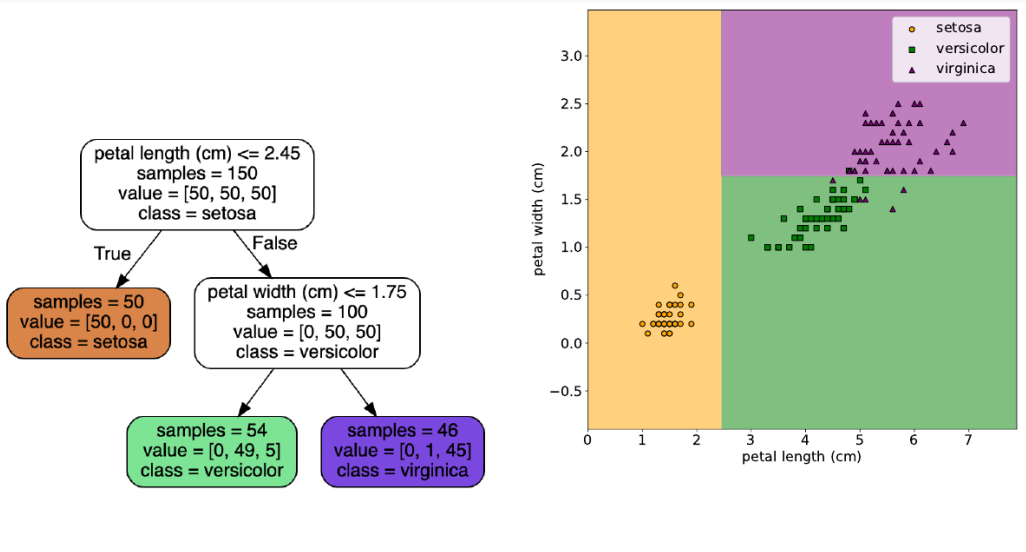
\includegraphics[width=0.98\textwidth]{Images/iris_decision_tree.PNG}
\caption{Decision tree per problema di classificazione specie di iris.}\label{fig:iris-decision-tree}
\end{figure}

\end{example}

\section{Richiami di probabilità}
Abbiamo diverse definizioni di probabilità.
\begin{description}
\item[Definizione Frequentistica] La probabilità di un evento è il rapporto tra il numero di casi favorevoli e il numero di casi possibili.
\item[Definizione Soggettiva] La probabilità di un evento è il prezzo che un individuo ritiene equo pagare per ricevere 1 se l'evento si verifica e 0 altrimenti.
\item[Definizione Bayesiana] La probabilità di un evento è l'\textit{incertezza} con cui l'evento si verifica.
\item[Definizione Assiomatica] Kolmogorov nel 1933 costruisce la teoria della probabilità a partire da degli assiomi.
\end{description}

L'incertezza può essere di due tipi:
\begin{description}
\item[aleatoria] ovvero è una \im{data uncertanty};
\item[epistemica] ovvero è una \im{model uncertanty};
\end{description}

\subsection{Proprietà della probabilità}
Chiamiamo $\pr(A)$ la probabilità dell'evento $A$, allora abbiamo le seguenti proprietà.

\begin{property}[Joint probability]
Se $A$ e $B$ sono due eventi indipendenti, allora:
\begin{equation}
\pr\pare{A\et B} \equiv \pr\pare{A, B} = \pr\pare{A} \cdot \pr\pare{B}.
\end{equation}
\end{property}

\begin{property}[Union probability]
Anche detta regola di unione esclusione. Se $A$ e $B$ sono due eventi indipendenti, allora:
\begin{equation}
\pr\pare{A\orr B} = \pr\pare{A} + \pr\pare{B} - \pr\pare{A\et B}.
\end{equation}
\end{property}

\begin{property}[Conditional probability]
\begin{equation}
\pr\pare{A\cond B} = \frac{\pr\pare{A, B}}{\pr\pare{A}}.
\end{equation}
Se i due eventi sono indipendenti questa si riduce a $\pr\pare{A\cond B} = \pr\pare{A}$.
\end{property}

\begin{property}[Conditional independece]
\begin{equation}
\pr\pare{A, B \cond C} = \pr\pare{A\cond C} \cdot \pr\pare{B\cond C}
\end{equation}
\end{property}

\subsection{Random variables}
Rappresentiamo con $X$ una variabile di cui non conosciamo il valore e la
chiamiamo \textit{variabile casuale} (\im{random variable}). Il set dei valori
che $X$ può assumere è detto \textit{spazio di sampling} (\im{sampling space}).
Un evento è dunque un set di risultati dato un sampling space definito.

Se la variabile è \textbf{discreta} abbiamo un sampling space numerabile e la PMF (\im{probability mass function}):
\begin{equation}
p\pare{x} \equiv \pr\pare{X = x}.
\end{equation}
Se invece la variabile è \textbf{continua} abbiamo un samplig space non numberabile e la CDF (\im{cumulative distribution function}):
\begin{equation}
P\pare{x} \equiv \pr\pare{X \leq x},
\end{equation}
da cui possiamo definire la PDF (\im{probability density function}):
\begin{equation}
p\pare{x} \equiv \deriv{}{x}P\pare{x},
\end{equation}
da cui segue:
\begin{align}
&\pr\pare{a \leq X \leq b} = \int_a^b p\pare{x} = P\pare{b} - P\pare{a} \\
&\Longrightarrow \pr\pare{x \leq X \leq x + dx} \approx p\pare{x}.
\end{align}
Se la CDF $P\pare{x}$ è monotona crescente allora la sua inversa $P^{-1}(q)$ è
detta \textit{quantile}. Il valore $x_q = P^{-1}\pare{q}$ è il valore per cui
$\pr\pare{X\leq x_q} < q$, ovvero il quantile $q$ della distribuzione $P$.

Se abbiamo due variabili casuali $X$ e $Y$ allora possiamo definire la \im{joint
distribution}:
\begin{equation}
p\pare{x, y} = p\pare{X = x, Y = y} \equiv p\pare{X = x\et Y = y}.
\end{equation}
Se le due variabili sono indipendenti e con cardinalità finita possiamo definire la \textit{distribuzione marginale} (\im{marginal distribution}) come:
\begin{equation}
p\pare{X = x} = \sum_y p\pare{X=x, Y=y},
\end{equation}
altrimenti se sono dipendenti la \textit{distribuzione condizionale} (\im{conditional distribution}) come:
\begin{equation}
\begin{split}
&p\pare{Y=y\cond X=x} = \frac{p\pare{X=x, Y=y}}{p\pare{X=x}} \\
&\Longrightarrow\quad p\pare{x, y} = p\pare{y\cond x}\cdot p\pare{x},
\end{split}
\end{equation}
da cui segue la \textbf{chain rule}:
\begin{equation}
p\pare{\ve{x}_{1,D}} = p\pare{x_1} p\pare{x_2\cond x_1} p\pare{x_3\cond x_1, x_2}\cdots p\pare{x_D\cond p_{1: D-1}}.
\end{equation}

Due variabili si dicono \im{marginalmente indipendenti} se
\begin{equation}
X\perp Y \quad\Longleftrightarrow\quad p\pare{X, Y} = p\pare{X} p\pare{Y},
\end{equation}
mentre si dicono \textbf{condizionalmente indipendenti} se
\begin{equation}
X\perp Y \quad\Longleftrightarrow\quad p\pare{X, Y\cond Z} = p\pare{X\cond Z} p\pare{Y\cond Z}. 
\end{equation}

\subsection{Momenti di una distribuzione}

\begin{definition}[Media] Definiamo \im{media} di una distribuzione come
\begin{equation}
\mathbb{E}\spare{X} \equiv \int_X x\, p\pare{x}dx \qquad\pare{ \mathbb{E}\spare{X_{\text{discreta}}} = \sum_{x\in X} x\, p\pare{x} }.
\end{equation}
La media è lineare, ovvero $\mathbb{E}\spare{\sum_{i=1}^n} = \sum_{i=1}^N \mathbb{E}\pare{X_i}$.
\end{definition}

\begin{definition}[Varianza] Definiamo \im{varianza} di una distribuzione come
\begin{equation}
\mathbb{V}\spare{X} \equiv \mathbb{E}\spare{\pare{X - \mu}^2},
\end{equation}
che con la definizione di prima possiamo anche scrivere come:
\begin{equation}
\begin{split}
\mathbb{V}\spare{X} &= \int_X \pare{x - \mu}^2\, p\pare{x}dx \\
&= \int x^2\, p\pare{x}dx \, +\, \mu^2\underbrace{\int p\pare{x}dx}_{=1} \, -\, 2\mu\underbrace{\int x\, p\pare{x}dx}_{=\mu} \\
&= \mathbb{E}\spare{X^2} - \mu^2.
\end{split}
\end{equation}
Con questa definizione è facile dimostrare l'identità
\begin{equation}
\mathbb{V}\spare{aX + b} = a^2\,\mathbb{V}\spare{X},
\end{equation}
inoltre anche la varianza è lineare, ma solo se le variabili sono indipendenti.
\end{definition}

\begin{definition}[Moda]
Definiamo \im{media} di una distribuzione il valore (o i valori) più probabile, ovvero
\begin{equation}
x^\star \;\text{t.c.}\; p\pare{x^\star} = \max p\pare{x},
\end{equation}
\end{definition}

Questi stimatori non danno tutta l'informazione contenuta nella distribuzione.

\subsection{Teorema di Bayes}

\begin{theorem}[Teorema di Bayes]\label{teo:bayes}
Data una quantità non nota $H$ (hypotesis) e dei dati noti $Y=y$ abbiamo che
\begin{equation}
p\pare{H=h\cond Y=y} = \frac{p\pare{H=h}p\pare{Y=y\cond H=h}}{p\pare{Y=y}}.
\end{equation}
\end{theorem}
Il teorema segue dall'identità $p\pare{h\cond y} p\pare{y} = p\pare{h} p\pare{y\cond h}$.
\begin{itemize}
\item $p\pare{h}$ viene detta \im{prior} ovvero ciò che conosciamo o assumiamo per $H$ \textit{prima} di fare qualunque misura;
\item $p\pare{y\cond h}$ è la \textit{distribuzione osservata} detta \im{likelihood}, è una funzione di $y$ ad $h$ fisso, ma non è un distribuzione di probabilità;
\item $p\pare{y}$ è detta \im{marginal likelihood}, indipendente da $h$, funge da costante di normalizzazione \[
p\pare{Y=y} = \sum_{h'\in H}p\pare{Y=y \cond H=h'} = \sum_{h'\in H}p\pare{H=h', Y=y};
\]
\item $p\pare{h\cond y}$ è detta \im{posterior distribution}.
\end{itemize}

\begin{example}[Monty Hall problem]
Posso scegliere una di tre porte. Dietro una delle porte c'è un premio. Inizio
con il scegliere la porta 1. Ho che la probabilità degli eventi $H_{1,2,3}$ che
il premio sia dietro la porta 1, 2 o 3 è
\[
p\pare{H_1} = p\pare{H=1} = \frac{1}{3}.
\]
Ora una delle porte non scelte da me si apre rivelando che dietro quella non c'è
il premio, in base a dove si trova il premio la probabilità degli eventi $Y_{2,
3}$ che si apra una porta o l'altra è data da $p\pare{Y=y, H=h}$:
\[
\begin{array}{l@{,\qquad}l@{,\qquad}l}
p\pare{Y=2, H_1} = \frac{1}{2} & p\pare{Y=2, H_2} = 0 & p\pare{Y=2, H_3} = 1, \\
\\
p\pare{Y=3, H_1} = \frac{1}{2} & p\pare{Y=3, H_2} = 1 & p\pare{Y=3, H_3} = 1. \\
\end{array}
\]
Si apre la porta 3. Mi viene data la scelta di cambiare porta prima che venga
rivelato dove si trova il premio, per massimizzare la probabilità di vittoria
posso calcolare le probabilità condizionate con Bayes. Dai calcoli di prima ho
che $p\pare(Y=3) = 1/6 + 1/3 = 1/3$ dunque:
\begin{equation}
\begin{split}
p\pare{H_1\cond Y=3} &= \dfrac{\frac{1}{3}\cdot\frac{1}{2}}{\frac{1}{2}} = \frac{1}{3}, \\
p\pare{H_2\cond Y=3} &= \dfrac{\frac{1}{3}\cdot 1}{\frac{1}{2}} = \frac{2}{3}, \\
p\pare{H_3\cond Y=3} &= 0, \\
\end{split}
\end{equation}
dunque mi conviene cambiare porta.
\end{example}

\subsection{Distribuzione di Gauss}
La distribuzione di Gauss (o gaussiana) è una tra le più usate in Machine Learning ed è definita come
\begin{equation}
\begin{split}
&P\pare{y} \equiv \pr\pare{Y\leq y},\qquad \pr\pare{a \leq Y \leq b} = P\pare{b} - \pare{a} \\
&\Phi\pare{y;\mu, \sigma^2} \equiv \int_{-\infty}^y \mathcal{N}\pare{\xi/\mu, \sigma^2}d\xi = \frac{1}{2}\spare{1 + \erf\pare{\frac{\xi}{\sqrt{2}}}},\quad \xi = \frac{y - \mu}{\sigma},
\end{split}
\end{equation}
ove $\erf$ è la \im{Gauss error function} definita come
\begin{equation}
\erf\pare{u} \equiv \frac{2}{\sqrt{\pi}} \int_0^\mu e^{-t^2}dt,
\end{equation}
mentre $\mathcal{N}$ è la PDF (probability density function) definita come
\begin{equation}
\mathcal{N}\pare{y\cond\mu,\sigma^2} \equiv \frac{1}{\sqrt{2\pi\sigma^2}}\exp\spare{-\frac{1}{2\sigma^2}\pare{y-\mu}^2}.
\end{equation}

Questa distribuzione è popolare per diversi motivi:
\begin{itemize}
\item dipende da soli due parametri ed entrambi sono di facile interpretazione;
\item per il teorema del limite centrale, nel limite $N\longrightarrow\infty$ ogni distribuzione può essere approssimata da una gaussiana;
\item rappresenta la somma di variabili causali indipendenti;
\item il numero di assunzioni è minimo.
\end{itemize}

\subsection{Altre distribuzioni notevoli}
Abbiamo:
\begin{itemize}
\item \im{t-Student} \begin{equation}
\tau\pare{y\cond\mu, \sigma^2, \nu} \propto \spare{1 + \frac{1}{\nu}\pare{\frac{y-\mu}{\sigma}}^2}^{-\frac{\nu+1}{2}}
\qquad\left\{\begin{array}{ll}
\mu & \text{mean} \\
\sigma & \text{mode} \\
\nu & \text{degree of formality} \\
\end{array}\right.;
\end{equation}
\item \im{Lorentz (Cauchy)} \begin{equation}
C\pare{x\cond\mu, \gamma} = \frac{1}{\gamma\pi}\spare{1 + \pare{\frac{x-\mu}{\gamma}}^2}^{-1};
\end{equation}
\item \im{Laplace} \begin{equation}
L\pare{y\cond\mu, b} = \frac{1}{2b}\exp\pare{-\frac{\left|y-\mu\right|}{b}}
\qquad\left\{\begin{array}{ll}
\mu & \text{mean} \\
\mu & \text{mode} \\
2b^2 & \text{variance} \\
\end{array}\right.;
\end{equation}
\item \im{beta} \begin{equation}
\Beta\pare{x\cond a, b} = \frac{1}{\beta\pare{a, b}}x^{a-1}\pare{1-x}^{b-1}
\qquad\left\{\begin{array}{ll}
\frac{a}{a+b} & \text{mean} \\
\pare{a-1}\pare{a+b-2} & \text{mode} \\
\frac{ab}{\pare{a+b}^2\pare{a+b+1}} & \text{variance} \\
\end{array}\right.;
\end{equation}
\item \im{gamma} \begin{equation}
\Ga\pare{x\cond a, b} = \frac{b^a}{\Gamma\pare{a}}x^{a-1}e^{-xb};
\end{equation}
\item \im{experimental} \begin{equation}
\Exp\pare{x\cond\lambda} = \Ga\pare{x\cond a=1, b=\lambda}
\end{equation}
\item \im{chi quadro} \begin{equation}
\chi^2_\nu\pare{x} = \Ga\pare{x\cond a=\frac{\nu}{2}, b=\frac{1}{2}}
\end{equation}
\end{itemize}
Alcune distribuzioni sono mostrate in \cref{fig:distributions}.

\begin{figure}
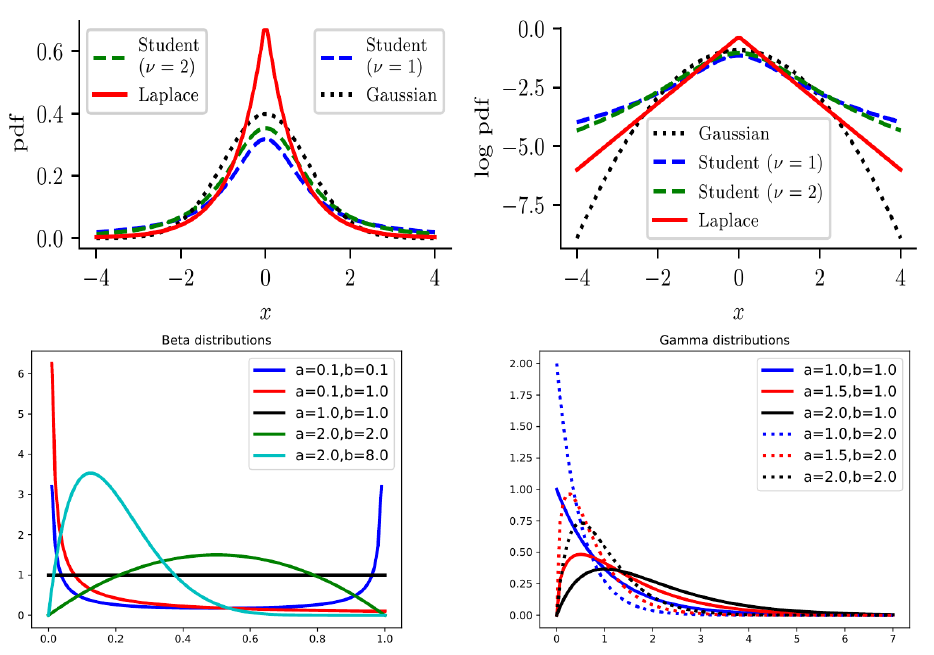
\includegraphics[width=0.98\textwidth]{Images/distributions.PNG}
\caption{Alcune distribuzioni notevoli.}\label{fig:distributions}
\end{figure}

\subsection{Osservazioni}
Supponiamo di avere due variabili causali descritte da distribuzioni gaussiane:
\begin{equation}
x_1 \sim \mathcal{N}\pare{\mu_1, \sigma_1^2},\qquad x_2 \sim \mathcal{N}\pare{\mu_2, \sigma_2^2},
\end{equation}
e di voler calcolare la PDF della loro somma $y = x_1 + x_2$, allora:
\begin{equation}
p\pare{y} = \mathcal{N}\pare{x_1\cond\mu_1, \sigma^2_1} \otimes \mathcal{N}\pare{x_2\cond\mu_2, \sigma^2_2} = \mathcal{N}\pare{y\cond\mu_1 + \mu_2, \sigma^2_1 + \sigma^2_2},
\end{equation}
ovvero \textit{la convoluzione di due gaussiane è una gaussiana}.

Supponiamo ora che $x$ sia una variabile casuale e $y = f\pare{x}$ una funzione
di essa. Talora è difficile calcolare $p\pare{y}$ analiticamente. Supponiamo ad
esempio che $x\sim\Unif\pare{-1,+1}$ e $y=x^2$, possiamo approssimare
$p\pare{y}$ con un generatore (uniforme) di numeri casuali e facendone il
quadrato per poi prendere la \im{distribuzione empirica}
\begin{equation}
p_S\pare{y} = \frac{1}{N_S}\sum_{x=1}^{N_S}\delta\pare{y-y_s}.
\end{equation}
Questo è detto \im{metodo monte carlo}.

\subsection{Modelli multivariati}
\begin{definition}[Covarianza]
Siano $X$ e $Y$ due variabili. La \im{covarianza} è
\begin{equation}
\Cov\spare{X, Y} \equiv \mathbb{E}\spare{\pare{X - \mathbb{E}\pare{E}}\pare{Y - \mathbb{E}\pare{E}}} = \mathbb{E}\spare{XY} - \mathbb{E}\spare{X}\mathbb{E}\spare{Y},
\end{equation}
ovvero una matrice $D$-dimensionale, con $D = \dim\pare{\ve{x}}$, che contiene le varianze sulla diagonale.
\end{definition}

\begin{definition}(Correlazione di Pearson)
La \im{correlazione di Pearson} tra le due variabili $X$ e $Y$ si definisce come
\begin{equation}
\rho \equiv \corr\spare{X, Y} = \frac{\Cov\spare{X, Y}}{\sqrt{\mathbb{V}\spare{X}\mathbb{V}\spare{Y}}}.
\end{equation}
\end{definition}

Possiamo scrivere
\begin{equation}
\Cov\spare{X} = \pare{\begin{array}{cccc}
\mathbb{V}\spare{X_1} & \Cov\spare{X_1, X_2} & \cdots & \Cov\spare{X_1, X_D} \\
\Cov\spare{X_2, X_1} & \mathbb{V}\spare{X_2} & \cdots & \Cov\spare{X_2, X_D} \\
\vdots & \vdots & \ddots & \vdots \\
\Cov\spare{X_D, X_1} & \Cov\spare{X_D, X_2} & \cdots & \mathbb{V}\spare{X_D} \\
\end{array}}
\end{equation}
e
\begin{equation}
\corr\pare{x} = \pare{\begin{array}{cccc}
1 & \frac{\mathbb{E}\spare{\pare{x_1-\mu_1}\pare{x_2-\mu_2}}}{\sigma_1\sigma_2} & \cdots & \frac{\mathbb{E}\spare{\pare{x_1-\mu_1}\pare{x_D-\mu_D}}}{\sigma_1\sigma_D} \\
\frac{\mathbb{E}\spare{\pare{x_2-\mu_2}\pare{x_1-\mu_1}}}{\sigma_2\sigma_1} & 1 & \cdots & \frac{\mathbb{E}\spare{\pare{x_2-\mu_2}\pare{x_D-\mu_D}}}{\sigma_2\sigma_D} \\
\vdots & \vdots & \ddots & \vdots \\
\frac{\mathbb{E}\spare{\pare{x_D-\mu_D}\pare{x_1-\mu_1}}}{\sigma_D\sigma_1} & \frac{\mathbb{E}\spare{\pare{x_D-\mu_D}\pare{x_2-\mu_2}}}{\sigma_D\sigma_2} & \cdots & 1 \\
\end{array}}.
\end{equation}

\subsubsection{Osservazioni}
\begin{itemize}
\item Il fatto che due variabili non siano correlate non vuol dire che siano indipendenti, tuttavia due variabili indipendenti sono necessariamente non correlate;
\item correlazione non implica causalità;
\item una correlazione che appare simile in diversi set di dati può sparire (o divenire opposta) se i dati sono combinati, questo è noto come \textit{Simpson's paradox}.
\end{itemize}

\subsection{Distribuzione gaussiana multivariata}
La definizione che abbiamo dato di distribuzione gaussiana si estende a più variabili. Innanzitutto definiamo la PDF
\begin{equation}
\mathcal{N}\pare{\ve{y}\cond\ve{\mu}, \Sigma} \equiv \frac{1}{\pare{2\pi}^{D/2}\left|\Sigma\right|^{1/2}}\exp\left\{-\frac{1}{2}\pare{\ve{y}-\ve{\mu}}^T\Sigma^{-1}\pare{\ve{y}-\ve{\mu}}\right\},
\end{equation}
dove $\Sigma = \Cov\spare{\ve{y}}$.

Supponiamo di avere due variabili aleatorie $\ve{y}_1$ e $\ve{y}_2$. Si può definire la distribuzione \im{jointly gaussian}. Con
\[
\ve{\mu} = \pare{\begin{array}{c}
\mu_1 \\
\mu_2
\end{array}},\qquad
\Sigma = \pare{\begin{array}{cc}
\Sigma_{11} & \Sigma_{12} \\
\Sigma_{21} & \Sigma_{22}
\end{array}},\qquad
\Lambda = \Sigma^{-1}
\]
le distribuzioni marginali sono
\begin{equation}
p\pare{\ve{y}_1} = \mathcal{N}\pare{\ve{y}_1\cond\ve{\mu}_1, \Sigma_{11}},\qquad p\pare{\ve{y}_2} = \mathcal{N}\pare{\ve{y}_2\cond\ve{\mu}_2, \Sigma_{22}}
\end{equation}
e la probabilità condizionata
\begin{equation}
p\pare{\ve{y}_1\cond\ve{y}_2} = \mathcal{N}\pare{\ve{y}_1\cond\ve{\mu}_{1\cond 2}, \Sigma_{1\cond 2}},
\end{equation}
con
\[
\ve{\mu}_{1\cond 2} = \ve{\mu}_1 + \Sigma_{12}\Sigma_{22}^{-1}\pare{\ve{y}_2 - \ve{\mu_2}},\qquad \Sigma_{1\cond 2} = \Sigma_{11} - \Sigma_{12}\Sigma_{22}^{-1}\Sigma_{21}=\Lambda_{11}^{-1},
\]
queste sono tutte gaussiane.

\section{Richiami di statistica}
Nella sezione precedente abbiamo assunto come noti i parametri $\ve{\theta}$,
in questa sezione impariamo come è possibile imparare questi parametri a partire
dai dati (training set) $\mathcal{D}$. Come abbiamo visto nell'\Cref{ex:iris},
il problema si riduce a trovare $\hat{\theta}$ tale che minimizzi il
misclassification rate, \Cref{eq:misclassification-rate}, ovvero:
\[
\hat{\theta} \quad\text{t.c.}\quad \mathcal{L}(\hat{\theta}) = \min\spare{\mathcal{L}\pare{\theta}} \equiv \min\spare{\frac{1}{N}\sum_{n=1}^N l\pare{y_n, f\pare{\ve{x_n}, \ve{\theta}}}}.
\]

\subsection{Maximum likelihood estimation (MLE)}
\begin{definition}[Maximum likelihood estimation]
Definitiamo la MLE, \im{maximum likelihood estimation}, come il valore di
$\theta$ che massimizza la probabilità condizionata di aver ottenuto il set di
dati $\mathcal{D}$, ovvero:
\begin{equation}
\hat{\theta}_{\text{MLE}} \equiv \argmax_{\ve{\theta}} p\pare{\mathcal{D}\cond\ve{\theta}}.
\end{equation}
Se i dati sono campioni indipendenti della stessa distribuzione, allora possiamo anche scrivere
\begin{equation}
p\pare{\mathcal{D}\cond\ve{\theta}} = \prod_{n=1}^N p\pare{\ve{y}_n \cond \ve{x}_n, \ve{\theta}}.
\end{equation}
Definiamo inoltre la NLL, \textsc{negative log-likelihood}, da usare come loss function come:
\begin{equation}
l\pare{\ve{\theta}} \equiv -\log p\pare{\mathcal{D}\cond\ve{\theta}} = -\sum_{n=1}^N \log p\pare{\ve{y}_n \cond \ve{x}_n , \ve{\theta}}.
\end{equation}
\end{definition}

Con queste definizioni abbiamo che la MLE è data
\begin{itemize}
\item per supervised learning da:
\begin{equation}
\hat{\theta}_{\text{MLE}} = \argmin_{\ve{\theta}} -\sum_{n=1}^N \log p\pare{\ve{y}_n \cond \ve{x}_n, \ve{\theta}};
\end{equation}
\item per unsupervised learning da:
\begin{equation}
\hat{\theta}_{\text{MLE}} = \argmin_{\ve{\theta}} -\sum_{n=1}^N \log p\pare{\ve{y}_n \cond \ve{\theta}}.
\end{equation}
\end{itemize}

Possiamo giustificare l'uso della MLE pensandola come un'approssimazione del \textit{posterior} Bayesiano dato un \textit{prior} uniforme.

\begin{example}
Se abbiamo
\[
p\pare{\ve{\theta}\cond\mathcal{D}} = \delta\pare{\ve{\theta}- \hat{\theta}_{\text{MAP}}}
\]
con $\hat{\theta}$ il posterior, allora
\[
\hat{\theta}_{\text{MAP}} = \argmin_{\ve{\theta}}-\log p\pare{\ve{\theta}\cond\mathcal{D}} = \argmin_{\ve{\theta}} -\log p\pare{\mathcal{D}\cond\ve{\theta}} -\log p\pare{\ve{\theta}},
\]
ed essendo $p\pare{\ve{\theta}} = 1$ abbiamo
\[
\pushQED{\qed}
\hat{\theta}_{\text{MAP}} = \argmin_{\ve{\theta}} -\log p\pare{\mathcal{D}\cond\ve{\theta}} = \hat{\theta}_{\text{MLE}}.\qedhere
\popQED
\]
\end{example}

\subsubsection{Distribuzione normale}
Supponiamo ora di avere una variabile casuale $Y$ distribuita normalmente, i.e.
$Y\sim \mathcal{N}\pare{\mu, \sigma^2}$, e sia $\mathcal{D} = \left\{ y_n \tc
n=1,\cdots,N \right\}$ un dataset con punti campionati indipendentemente,
allora:
\begin{equation}
\begin{split}
\NLL\pare{\mu, \sigma^2} &= -\sum_{n=1}^{N_D}\log\spare{\pare{\frac{1}{2\pi\sigma^2}}^\HALF \exp\pare{-\frac{1}{2\sigma^2}\pare{y_n-\mu}^2}} \\
&=\frac{1}{2\sigma}\sum_{n=1}^{N_D}\pare{y_n - \mu}^2 + \frac{N_D}{2}\log\pare{2\pi\sigma^2}.
\end{split}
\end{equation}
Ora estremizzando otteniamo
\begin{align}
\pderiv{}{\mu}\NLL\pare{\mu, \sigma^2} = 0 &\;\Longleftrightarrow\; \hat{\mu}_{\MLE} = \frac{1}{N_D}\sum_{n=1}^{N_D} y_n = \bar{y}\\
\pderiv{}{\sigma^2}\NLL\pare{\mu, \sigma^2} = 0 &\;\Longleftrightarrow\; \hat{\sigma}^2_\MLE = \frac{1}{N_D}\sum_{n=1}^{N_D}\pare{y_n - \hat{\mu}_\MLE}^2 = \frac{1}{N_D}\sum_{n=1}^{N_D}y_n^2 - \bar{y}^2 = s^2 - \bar{y}^2.
\end{align}

\subsubsection{Distribuzione normale multivariata}
Per una distribuzione multivariata i risultati sono analoghi. Abbiamo
\begin{equation}
l\pare{\ve{\mu}, \Sigma} = \log p\pare{\mathcal{D}\cond\ve{\mu},\Sigma} = \frac{N_D}{2}\log\left|\Lambda\right| = -\HALF\sum_{n=1}^{N_D}\pare{\ve{y}_n - \ve{\mu}}^T \Lambda\pare{\ve{y}_n - \ve{\mu}}
\end{equation}
dove $\Lambda = \Sigma^{-1}$ è la \im{precision matrix}. Dall'estremizzazione
segue, come prima, l'empirical mean $\hat{\ve{\mu}}$ e l'empirical covariance
matrix $\hat{\Sigma}$:
\begin{align}
\hat{\ve{\mu}} &= \frac{1}{N_D}\sum_{n=1}^{N_D}\ve{y_n} = \bar{\ve{y}} \\
\hat{\Sigma} &= \frac{1}{N_D}\sum_{n=1}^{N_D}\pare{\bar{\ve{y}}_n - \bar{\ve{y}}}\pare{\bar{\ve{y}}_n - \bar{\ve{y}}}^T 
\end{align}

\subsection{Empirical risk minimization (ERM)}
La MLE può essere generalizzata sostituendo la loss function logaritmica NLL con qualunque altra funzione $l$:
\begin{equation}
\mathcal{L}\pare{\ve{\theta}} = \frac{1}{N}\sum_{n=1}^N l\pare{\ve{y}_n, \ve{\theta}; \ve{x}_n}.
\end{equation}
Questo processo di cambiare loss function è noto come ERM, \im{empirical risk minimization}. %% ???

\begin{example}[ERM per problema di classificazione]
In un problema di classificazione avremo una loss function
\begin{equation}
l_{01}\pare{\ve{y}_n, \ve{\theta}; \ve{x}_n} = \left\{\begin{array}{l@{\quad\text{se}\quad}l}
1 & \ve{y}_n = f\pare{\ve{x}_n; \ve{\theta}} \\
0 & \ve{y}_n \neq f\pare{\ve{x}_n; \ve{\theta}} 
\end{array}\right.
\end{equation}
dove $f\pare{\ve{x}, \ve{\theta}}$ è un predittore. L'empirical risk diviene
\begin{equation}
\mathcal{L}\pare{\ve{\theta}} = \frac{1}{N}\sum_{n=1}^N l_{01}\pare{\ve{y}_n, \ve{\theta}; \ve{x}_n},
\end{equation}
che è il misclassification rate nel training set. In problemi binari possiamo
riscrivere il misclassification rate usando l'indicatore binario come definito
in \eqref{eq:indicatore-binario}. Se $\tilde{y} \in \left\{ -1, +1 \right\}$ è
il time label e $\hat{y}\in \left\{-1, +1\right\} = f\pare{\ve{x},
\ve{\theta}}$ la prediction, allora:
\begin{equation}
l_{01}\pare{\tilde{y}, \hat{y}} = \mathbb{I}\pare{\tilde{y}\neq\hat{y}} = \mathbb{I}\pare{\tilde{y}\hat{y}<0},
\end{equation}
con cui il rischio empirico si scrive
\begin{equation}
\mathcal{L}\pare{\ve{\theta}} = \frac{1}{N}\sum_{n=1}^{N}l_{01}\pare{\tilde{y}_n, \hat{y}_n} = \frac{1}{N}\sum_{n=1}^N\mathbb{I}\pare{\tilde{y}_n\hat{y}_n < 0}.
\end{equation}
La funzione $l_{01}$ è però problematica in quanto non-smooth e quindi difficile
da ottimizzare. In questi casi si può utilizzare una funzione surrogata,
definita generalmente come limite superiore convesso, ad esempio
\begin{equation}
l_{ll}\pare{\tilde{y}, \eta} = -\log{p\pare{\tilde{y}\cond\eta}} = \log\pare{1 + e^{-\tilde{y}\eta}},\qquad p\pare{\tilde{y}\cond\ve{x},\ve{\theta}} = \sigma\pare{\hat{y}\eta} = \frac{1}{1+e^{-\hat{y}\eta}}
\end{equation}
\end{example}

\subsection{Altri metodi di minimizzazione}

\subsubsection{Metodo dei momenti}
Il calcolo di $\nabla_{\ve{\theta}}\NLL\pare{\ve{\theta}} = 0$, ovvero la
ricerca dei punti estremi, può essere difficile. Il metodo dei momenti consiste
nell'eguagliare i momenti teorici della distribuzione ai momenti empirici,
ovvero:
\begin{equation}
\left.
\begin{array}{ll}
\textsc{Momenti teorici:} & \mu_k = \mathbb{E}\spare{Y^k} \\
\\
\textsc{Momenti empirici:} & \hat{\mu}_k = \frac{1}{N}\sum_{n=1}^N y_n^k
\end{array}
\right\} \mu_k = \hat{\mu}_k \quad\Longrightarrow\quad \text{ho } k \text{ equazioni}.
\end{equation}
Ad esempio per la gaussiana abbiamo:
\begin{align*}
&\mu_1 = \mu = \bar{y}, \\
&\mu_2 = \sigma^2 + \mu^2 = s^2.
\end{align*}
In questo caso abbiamo che MOM \(=\) MLE, ma questo non è vero in generale (ad
esempio non è vero per la distribuzione uniforme).

\subsubsection{Online recursive estimation}
Se tutto il dataset $\mathcal{D}$ è noto e disponibile prima che inizi il
processo di learning si dice che si fa \im{batch learning}. In alcuni casi però
il dataset è disponibile in blocchi e si dice che si fa \im{online learning}. Si
ha che $\hat{\ve{\theta}}_{t-1}$ è la predizione dato il blocco
$\mathcal{D}_{1:t-1}$, quello che vogliamo fare è trovare $\ve{\theta}_t =
f(\hat{\ve{\theta}}_{t-1}, \ve{y}_t)$ con un update ricorsivo.

\begin{definition}[Moving average]
Per una gaussiana multivariata si può definire la \im{media mobile} come:
\begin{equation}
\begin{split}
\hat{\ve{\mu}}_t &= \frac{1}{t}\sum_{n=1}^t\ve{y}_n \\
&= \frac{1}{t}\spare{\pare{t-1}\hat{\ve{\mu}}_{t-1} + \ve{y}_t} = \hat{\ve{\mu}}_{t-1} + \frac{1}{t}\pare{\ve{y}_t - \hat{\ve{\mu}}_{t-1}}.
\end{split}
\end{equation}
Nel caso in cui la distribuzione cambi in modo continuo la moving average può
anche essere pesata.
\end{definition}

\subsection{Regolarizzazione}
Un problema della MLE (maximum likelihood estimation) e della ERM (empirical
risk minimization) è che i parametri tendono ad essere determinati minimizzando
il loss nel training set, ma non necessariamente lo minimizzano per i dati
futuri. Per ridurre l'entità del problema si può procedere con la
regolarizzazione:
\begin{equation}
\mathcal{L}\pare{\ve{\theta}, \lambda} = \Bigl[ \underbrace{\frac{1}{N}\sum_{n=1}^N l\pare{\ve{y}_n, \ve{\theta}; \ve{x}_n}}_{\mathcal{L}\pare{\ve{\theta}}} + \lambda C\pare{\ve{\theta}} \Bigr],
\end{equation}
dove $\lambda$ è detto \im{regularization parameter} e $C\pare{\ve{\theta}}$ è
la \im{penality function}, ad esempio si può avere:
\[
C\pare{\ve{\theta}} = -\log{p\pare{\ve{\theta}}}.
\]

Per \(\lambda = 1\) e riscalando \(p\pare{\ve{\theta}}\) si ha la NLL:
\begin{equation}
\NLL\pare{\ve{\theta}, \lambda} = - \spare{\sum_{n=1}^N\log{p\pare{\ve{y}_n\cond\ve{x}_n,\ve{\theta}}} + \log{p\pare{\ve{\theta}}}} = -\spare{\log{p\pare{\mathcal{D}\cond\ve{\theta}}} + \log{p\pare{\ve{\theta}}}},
\end{equation}
che implica:
\begin{equation}
\hat{\ve{\theta}} = \argmax_{\ve{\theta}}\log{p\pare{\ve{\theta}\cond\mathcal{D}}} = \argmax_{\ve{\theta}}\spare{\log{p\pare{\mathcal{D}\cond\ve{\theta}}} + \log{p\pare{\ve{\theta}}} - \text{const}}.
\end{equation}
Questa stima si chiama MAP (\im{maximum a posterior}) estimation.


\subsubsection{Come scegliere \(\lambda\)}
Un valore (troppo) piccolo per \(\lambda\) equivale a minimizzare il rischio
empirico (\im{overfitting}); un valore (troppo) grande equivale a essere troppo
vicini al prior (\im{underfitting}). Una soluzione è dividere il training set in
due classi: una di training ($\mathcal{D}_{\text{train}},\,80\%$) ed una di
validation ($\mathcal{D}_{\text{val}},\,20\%$). Si va quindi a fittare il
modello su $\mathcal{D}_{\text{train}}$ per ogni setting $\lambda$ e poi a
valutare la performance del modello ottenuto su $\mathcal{D}_{\text{val}}$. Si
prende dunque il valore di $\lambda$ per cui si è ottenuta la performance
migliore.

\begin{definition}[Regularized empirical risk]
Definiamo l'\im{empirical risk regolarizzato} come:
\begin{equation}
R_\lambda\pare{\ve{\theta}, \mathcal{D}} \equiv \frac{1}{\left|\mathcal{D}\right|}\sum_{\pare{\ve{x}, \ve{y}}\in\mathcal{D}} l\pare{\ve{y}, f\pare{\ve{x}, \ve{\theta}}} + \lambda C\pare{\theta}
\end{equation}
\end{definition}
\noindent
Il processo che seguiamo è quindi il seguente:
\begin{enumerate}
\item costruiamo il modello: $\hat{\ve{\theta}}_\lambda\pare{\mathcal{D}_\text{train}} = \argmin_{\ve{\theta}} R_\lambda\pare{\ve{\theta}, \mathcal{D}_{\text{train}}}\;\forall\lambda$;
\item calcoliamo il validation risk: $R_\lambda^\text{val} = R_0\pare{\hat{\ve{\theta}}_\lambda\pare{\mathcal{D}_\text{train}}, \mathcal{D}_\text{val}}$;
\item prendiamo il \(\lambda\) che ha dato la miglior performance: \(\lambda^\star = \argmin_{\lambda\in S} R_\lambda^\text{val}\);
\item si ri-fitta il modello su \(\mathcal{D} = \mathcal{D}_\text{train}\cup\mathcal{D}_\text{val}\) usando \( \lambda=\lambda^\star \);
\item si ottengono i parametri \(\hat{\ve{\theta}}^\star = \argmin_{\ve{\theta}} R_{\lambda^\star}\pare{\ve{\theta}, \mathcal{D}}\).
\end{enumerate}

    Se il dataset è piccolo, eliminare il \( 20\% \) dei dati può essere dannoso e si procede quindi con la \im{cross validation}. Questa consiste nel dividere il dataset in $K$ \im{fold} e per ognuno allenare il modello su tutti i fold meno il \(k\)-esimo, il quale viene usato come test fold. Si definisce l'empirical risk regolarizzato per cross validation:
    \begin{equation}
    R_\lambda^\text{CV} \equiv \frac{1}{K} \sum_{k=1}^K R_0\pare{\hat{\ve{\theta}}_\lambda\pare{\mathcal{D} - \mathcal{D}_k}, \mathcal{D}_k}
    \end{equation}

\subsection{Statistica Bayesiana}
    Abbiamo ora visto diversi metodi per determinare i parametri a partire dei dati, ma dobbiamo
    ancora parlare della loro incertezza. Il \Crefn{teo:bayes} ci aiuta in questo, infatti:
    \begin{equation}
        p\pare{\ve{\theta}\cond \mathcal{D}} = \frac{p\pare{\ve{\theta}} p\pare{\mathcal{D}\cond\ve{\theta}}}{p\pare{\mathcal{D}}} = \frac{p\pare{\ve{\theta}} p\pare{\mathcal{D}\cond\ve{\theta}}}{\int p\pare{\ve{\theta}'}p\pare{\mathcal{D}\cond\ve{\theta}'}d\ve{\theta}'}
    \end{equation}

    dove \(\mathcal{D} = \{ \left( \ve{x}_n, \ve{y}_n \right) \} \) per supervised learning
    e \(\mathcal{D} = \{ \left( \ve{y}_n \right) \} \) per unsupervised learning, \(n = 1,\ldots, N \).

    Una voltache il posterior sui paramentri è stato determinato, possiamo calcolare il posterior
    della distribuzione predittiva marginalizzando su \(\ve{\theta}\):
    \begin{equation}
        p \left( \ve{y}\cond\ve{x}, \mathcal{D} \right) = \int p \left( \ve{y}\cond\ve{x}, \theta \right) p \left( \ve{\theta}\cond\mathcal{D} \right) d\theta,
    \end{equation}
    questo è noto come BMA (\im{Bayes model averaging}).

    Consideriamo una distribuzione gaussiana di cui sia nota la varianza, nel caso univariato la
    likelihood per \(\mu\) ha la forma
    \begin{equation}
        p \left( \mathcal{D}\cond\mu \right) \propto \exp \left\{ - \frac{1}{2\sigma} \sum_{n=1}^{N_D} \left( y_n - \mu \right)^2 \right\}.
    \end{equation}
    Si può mostrate che il prior coniugato è un'altra gaussiana
    \(\mathcal{N}\left( \mu\cond\check{m}, \check{\tau}^2 \ \right)\) e usando il \Crefn{teo:bayes} troviamo che il
    posterior è
    \begin{equation}
        \begin{split}
            &p \left( \mu\cond\mathcal{D}, \sigma^2 \right) = \mathcal{N} \left( \mu\cond\hat{m}, \hat{\tau}^2 \right) \\
            &\text{dove}\;
                \left\{\begin{array}{ll}
                    \hat{\tau}^2 &= \frac{1}{\frac{N}{\sigma^2} + \frac{1}{\check{\tau}^2}} = \frac{\sigma^2\check{\tau}^2}{N\check{\tau}^2 + \sigma^2} \\
                    \hat{m} &= \hat{\tau}^2 \left( \frac{\check{m}}{\check{\tau}^2} + \frac{N\bar{y}}{\sigma^2} \right) = \frac{\sigma^2}{N\check{\tau}^2 + \sigma^2}\check{m} + \frac{N\check{\tau}^2}{N\check{\tau}^2 + \sigma^2}\bar{y}                    
                \end{array}\right.
        \end{split}
    \end{equation}
    e con \(\bar{y}\equiv\frac{1}{N}\sum_{n=1}^N y_n\) la media empirica.
    Definendo ora \(\kappa = 1/\sigma^2\) e \(\check{\lambda} = 1/\check{\tau}^2\) posso scrivere:
    \begin{equation}
        \begin{split}
            \hat{\lambda} &= \check{\lambda} + N\kappa \\
            \hat{m} &= \frac{N\kappa\bar{y} + \check{\lambda}\check{m}}{\hat{\lambda}} = \frac{N\kappa}{N\kappa + \check{\lambda}}\bar{y} + \frac{\check{\lambda}}{N\kappa + \check{\lambda}}\check{m}
        \end{split}.
    \end{equation}

    La precisione del posterior \(\hat{\lambda}\) è dunque la precisione del prior \(\check{\lambda}\)
    più \(N\) unità di misura di precisione \(\kappa\). La media del posterior (\(\hat{m}\)) è invece
    una combinazione convessa della media empirica \(\bar{y}\) e della media del prior \(\check{m}\).
    Consideriamo ora il posterior dopo aver visto un singolo dato \(y\) (i.e. abbiamo \(N = 1\)),
    si ha che la \im{posteriori mean} può essere data in tre modi:
    \begin{equation}
        \hat{m} = \underbrace{\frac{\check{\lambda}}{\hat{\lambda}}\check{m} + \frac{\kappa}{\hat{\lambda}}\bar{y}}_{\substack{\text{convex combination}\\ \text{of prior and data}}}
        = \underbrace{\check{m} + \frac{\kappa}{\hat{\lambda} \left( \bar{y} - \check{m} \right)}}_{\substack{\text{prior mean adjusted}\\ \text{to data}}}
        = \underbrace{\bar{y} = \frac{\check{\lambda}}{\hat{\lambda}}\left( \bar{y} - \check{m} \right)}_{\substack{\text{data adjusted to} \\ \text{the prior mean}}}
    \end{equation}
    ed abbiamo lo \im{standard error}:
    \begin{equation}
        \operatorname{se} \left( \mu \right) = \sqrt{\mathbb{V}\left[ \mu \left[ \mathcal{D} \right] \right]}.
    \end{equation}

    Se uso un \textit{uninformative prior} per \(\mu\) ponendo \(\check{\lambda} = 0\), allora \(\hat{m} = \bar{y}\).
    Supponendo di approssimare \(\sigma^2 \sim s^2 \equiv \frac{1}{N}\sum_{n=1}^N \left( y_n - \bar{y} \right)^2\) segue che
    \begin{equation}
        \hat{\lambda} = N\kappa = \frac{N}{s^2} \quad \Longrightarrow \quad \operatorname{se} \left( \mu \right) = \frac{1}{\sqrt{\lambda}} = \frac{s}{\sqrt{N}}.
    \end{equation}
    Ovvero abbiamo che l'incertezza decresce ad un rateo di \(1/\sqrt{N}\).

    \begin{observation}
        Quando non abbiamo informazioni sul prior è desiderabile usare un prior uninformative.
        Ad esempio un flat prior, i.e. \(p \left( \mu \right) = 1 \).
    \end{observation}

    \begin{observation}
        Qualunque modello Bayesiano richiede di specificare un prior \(p \left( \theta \right)\) per i parametri.
        I parametri del prior sono detti \textbf{iperparametri} e sono denotati con \(\Phi\). Se non
        sono noti possiamo mettrci sopra un prior (multi-level model \(\Phi\rightarrow\theta\mathcal{D}\)) e
        definire la joint distribution \(p \left( \ve{\phi}, \ve{\theta}, \mathcal{D} \right) = p \left( \ve{\Phi} \right) p \left( \ve{\theta} \cond \ve{\Phi}\right) p \left( \mathcal{D} \cond \theta \right)\).
    \end{observation}

    \begin{table}[]
        \centering\begin{tabular}{ll}
            \toprule
            Method & Definition \\
            \midrule
            MLE & \( \hat{\ve{\theta}} = \argmax_{\ve{\theta}} p \left( \mathcal{D}\cond \theta \right) \) \\
            MAP & \( \hat{\ve{\theta}} = \argmax_{\ve{\theta}} p \left( \mathcal{D}\cond \theta \right) p \left( \ve{\theta} \cond \ve{\Phi} \right)\) \\
            Full Bayes & \( p \left( \ve{\phi}, \ve{\theta}, \mathcal{D} \right) \propto p \left( \ve{\Phi} \right) p \left( \ve{\theta} \cond \ve{\Phi}\right) p \left( \mathcal{D} \cond \theta \right) \) \\
            \bottomrule
        \end{tabular}
        \caption{Metodi visti per ottenere i parametri.}\label{tab:metodi-parametri}
    \end{table}

\subsection{Intervalli credibili e di confidenza}
    Una distribuzione posteriore è un oggetto multidimensionale difficile da
    visualizzare e da trattere. Può essere quindi utile calcolare degli
    stimatori puntuali, come la media e moda posteriore, per determinare un
    intervallo di credibilità che quantifichi l'incertezza associata alle stime.

    \begin{definition}[Intervallo di credibilità]
        L'\im{intervallo di credibilità} \( 100\left( 1 - \alpha \right)\% \) è la regione \(C = \left( l, u \right)\)
        che contiene \( 1 - \alpha \) della probabilità posteriore, ovvero:
        \begin{equation}
            C_\alpha \left( \mathcal{D} \right) = \left( l, u \right) \tc P\left( l \leq \theta \leq u \cond \mathcal{D} \right) = 1 - \alpha
        \end{equation}
        dove \(l\) si dice \textit{lower} e \(u\) \textit{upper}. Inoltre se il posterior
        ha una PDF nota, allora \(l = F^{-1} \left( \alpha/2 \right) \) e \( u = F^{-1} \left( 1 - \alpha/2 \right)\),
        ove \(F\) è la CDF del posterior.
    \end{definition}

    \begin{definition}[Intervallo di confidenza]
        Si dice \im{intervallo di confidenza} \(100 \left( 1 - \alpha \right)\% \), per la stima di un
        parametro \( \theta \), la regione \(I ( \tilde{\mathcal{D}} ) = ( l( \mathcal{\tilde{D}} ), u( \mathcal{\tilde{D}} ) )\)
        ottenuto da un data set \(\mathcal{D}\) tale che
        \begin{equation}
            \pr \left( \theta \in I \left( \mathcal{\tilde{D}} \cond \mathcal{D} \sim \theta \right) \right) = 1 - \alpha.
        \end{equation}

    \end{definition}

    \begin{observation}
        L'intervallo di credibilità è un concetto Bayesiano mentre l'intervallo di
        confidenza è un concetto frequentista. CL (frequentista): \( \theta \) è una costante fissa
        non nota e i dati sono aleatori. CI (Bayesiano): i dati sono fissi perchè noti,
        \( \theta \) è invece ignota. Un CL al \( 95\% \) \underline{non} significa che il
        parametro stia verosimilmente dentro l'intervallo il \( 95\% \) delle volta dati
        i dati osservati.
    \end{observation}

    \begin{example}
        Supponiamo di generare due interi \( \mathcal{D} = \left( y_1, y_2 \right) \) da:
        \[
            p \left( y\cond \theta \right) = \left\{
            \begin{array}{l@{\quad\text{se}\quad}l}
                0.5 & y = \theta \\
                0.5 & y = \theta + 1 \\
                0 & \text{altrimenti} \\
            \end{array}\right..
        \]
        Se \( \theta = 39 \) possiamo ottenere i seguenti risultati:
        \[
            \left( 39, 39 \right), \left( 39, 40 \right), \left( 40, 39 \right), \left( 40, 40 \right).
        \]
        Sia \( m = \min \left( y_1, y_2 \right) \) e l'intervallo
        \( \left[ l(\mathcal{D}), U(\mathcal{D}) \right] = [m, m] \). Segue che i possibili intervalli
        sono:
        \[
            [39, 39], [39, 39], [39, 39], [40, 40]
        \]
        e dunque l'intervallo definito risulta in un CI \( 75\% \) per \( \theta = 39\).
        Se però osserviamo \( \mathcal{D} = \left( 39, 40 \right) \) allora
        \( p \left( \theta=39 \cond \mathcal{D} \right) \), ma CI è solo \( 75\% \). Il CI fallisce per esperimenti
        \underline{non} ripetibili.
    \end{example}

\subsection{Bias-variance tradeoff}
    Sia \( \hat{\theta} \) lo stimatore statistico e \( \hat{\theta} \left( \mathcal{D} \right) \) l'estimando. Nel formalismo
    frequentista i dati sono variabili casuali campionati da una distribuzione
    \( p^\star \left( \mathcal{D} \right)\), che induce una distribuzione sull'estimendo
    \( p^\star \left( \hat{\theta} \left( \mathcal{D} \right) \right) \).

    \begin{definition}[Bias]
        Il \im{bias} di uno stimatore \( \hat{\theta} \) è definito come:
        \begin{equation}
            \bias \left( \theta(\cdot) \right) \equiv \mathbb{E} \left[ \hat{\theta} \left( \mathcal{D} \right) \right] - \theta^\star
        \end{equation}
        dove \( \theta^\star \) è il valore vero. Se il bias è nulla, lo stimatore viene detto
        \im{unbiased}.
    \end{definition}

    Per una gaussiana abbiamo:
    \begin{align}
        & \bias \left( \hat{\mu} \right) = \mathbb{E} \left[\bar{x}\right] - \mu = \mathbb{E} \left[ \frac{1}{N_D}\sum_{n=1}^{N_D} x_n \right] - \mu = \frac{N_D \mu}{N_D} - \mu = 0  \quad \Longrightarrow \quad \text{Unbiased},  \\
        & \bias \left( \hat{\sigma}^2 \right) = \mathbb{E} \left[ s^2 \right] - \sigma^2 = \frac{N_D - 1}{N_D}\sigma^2 - \sigma^2 \neq 0  \quad \Longrightarrow \quad \text{Biased}.
    \end{align}
    Possiamo però definire una versione unbiased della varianza come:
    \begin{equation}
        \sigma^2_{\text{unb}} = \frac{1}{N_D - 1}\sum_{n=1}^{N_D} {\left( x_n - \bar{x} \right)}^2 = \frac{N_D}{N_D - 1}\sigma^2_{\MLE}
    \end{equation}

    \begin{definition}[Varianza di uno stimatore]
        La \im{varianza di uno stimatore} è
        \begin{equation}
            \mathbb{V} ( \hat{\theta} ) \equiv \mathbb{E} ( \hat{\theta}^2 ) - {( \mathbb{E} [ \hat{\theta} ] )}^2
        \end{equation}
    \end{definition}

    Idealmente vogliamo avere una varianza minima per tutti gli stimatori. Il seguente
    teorema fornisce un limite minimo alla varianza.

    \begin{theorem}[Disuguaglianza di Cramér-Rao]
        Per uno stimatore \underline{unbiased} \( \theta^\star \) si ha che:
        \begin{equation}
            \mathbb{V} \left[ \hat{\theta} \right] \geq \frac{1}{NF(\theta^\star)},
        \end{equation}
        ove \( F(\theta^\star) \) è la \textit{Fisher information}.
    \end{theorem}

    Si può dimostrare che la MLE raggiunge il bond imposto da Cramér-Rao. Sia
    \( \hat{\theta} = \hat{\theta} \left( \mathcal{D} \right) \) l'estimato e \(
    \bar{\theta} = \mathbb{E} \left[ \hat{\theta} \right] \) il valore di
    aspettazione corrsispondente (tutti da \(p \left(
    \mathcal{D}\cond\theta^\star \right) \)), allora:

    \begin{equation}
        \begin{split}
            \mathbb{E} \left[ {\left( \hat{\theta} - \theta^* \right)}^2 \right] &= \mathbb{E} \left[ {\left[ ( \hat{\theta} - \bar{\theta} ) + ( \bar{\theta} - \theta^\star )\right]}^2 \right] \\
            &= \mathbb{E} \left[ {\left( \hat{\theta} - \bar{\theta} \right)}^2 \right] + 2\mathbb{E} \left[ {\left( \hat{\theta}-\bar{\theta} \right)}^2 \right] + 2\left( \bar{\theta} - \theta^\star \right)\mathbb{E} \left[ \hat{\theta} - \theta^\star \right] + {\bar{\theta}-\theta^\star}^2 \\
            &= \mathbb{E} \left[ {\left( \hat{\theta} - \bar{\theta} \right)}^2 \right]  + {\left( \bar{\theta} - \theta^\star \right)}^2 = \mathbb{V}\left[\hat{\theta}\right] + \bias^2 \left( \hat{\theta} \right)
        \end{split}
    \end{equation}

    \begin{example}
        Supponiamo di stimare la media di una distribuzionne gaussiana a partire dai dati
        \mbox{\( \ve{x} = \left( x_1, \ldots, x_n \right) \)} assumendo che questi siano stati campionati da
        \( x_n \sim \mathcal{N} \left( \theta^\star = 1, \sigma^2 \right) \). Uno stimatore ovvio è dato dalla MLE
        che ha bias nullo e varianza \( \mathbb{V} [\bar{x}/\theta^\star] = \sigma^2/N \).
        Possiamo dare uno stimatore MAP sotto un prior gaussiano, in tal caso:
        \[
            \tilde{x} = \frac{N}{N + \kappa_0} \bar{x} + \frac{\kappa_0}{N + \kappa_0}\theta_0 = w\bar{x} + \left( 1-w \right) \theta_0
        \]
        con prior \( \mathcal{N} \left( \theta_0, \sigma^2 / \kappa_0 \right) \). Allora abbiamo:
        \begin{align*}
            &\mathbb{E}_{\text{MAP}} \left[ \tilde{x} \right] - \theta^\star = w\theta^\star + (1 - w)\theta_0 - \theta^\star = \left( 1-w \right) \left( \theta_0 - \theta^\star \right),  \\
            &\mathbb{V}_{\text{MAP}} \left[ \tilde{x} \right] = w^2\frac{\sigma^2}{N} < \mathbb{V}_\text{MLE} .\left[ \hat{x} \right],
        \end{align*}
        ovvero è uno stimatore biased essendo \( 0 < w < 1\).
    \end{example}

\section{Ottimizzazione}
    Abbiamo viesto nelle precedenti lezioni che il machine learning ha come
    obbiettivo quello di stimare dei parametri \( \ve{\theta} \) (o degli iperparametri
    \( \Phi \)) di un modello, ovvero determinare i valori di best-fit e relativi
    intervalli di credibilità. Questo si realizza minimizzando una funzione
    scalare, la less function
    \[
        \mathcal{L}: \Theta\rightarrow\mathbb{R},
    \]
    dove \( \theta\in\Theta \), per trovare:
    \[
        \theta^* = \argmin_{\ve{\theta}} \mathcal{L}\left( \ve{\theta} \right) \quad\text{o meglio}\quad
        \hat{\theta}=\argmin_{\ve{\theta}} \mathcal{L}\left[ \ve{\theta} \right] \quad\text{per}\;
        \theta^\star \sim \hat{\theta}.
    \]

    Assumiamo per semplicità che \( \Theta \subseteq \mathbb{R}^D \), con \(D\) il numero
    delle variabili ottimizzate, in questo modo abbiamo che l'ottimizzazione
    è \textbf{continua}.

    \begin{observation}
        Lo spazio dei parametri è tale che può esistere un solo minimo globale o
        più minimi globali, oltre ad una serie di minimi locali. Il punto di
        minimo è computazionalmente \textit{sempre in termini locali}, i.e.:
        \[
            \exists \delta > 0 ,\; \forall\ve{\theta}\in\Theta  \quad\tc\quad
            || \ve{\theta} - \hat{\ve{\theta}} || < \delta ,\;
            \mathcal{L} (\hat{\ve{\theta}}) < \mathcal{L} (\ve{\theta}).
        \]
        un minimo locale può essere circondato da minimi simili (flat direction).
        Un algoritmo che converge ad un punto stazionario è detto
        \im{globally convergent}.
    \end{observation}

    \begin{observation}
        Per loss function che sono due volte differenziabili possiamo considerare
        il vettore gradiente \( g\left( \ve{\theta} \right) = \nabla\mathcal{L}\left( \ve{\theta} \right) \) e
        la matrice Hessiana \( H\left( \ve{\theta} \right)  = \nabla^2 \mathcal{L}\left( \ve{\theta} \right) \).
        Per un punto \( \hat{\ve{\theta}} \in \mathbb{R}^D \), indicando \( \hat{g} = g\left( \ve{\theta} \right)|_{\hat{\ve{\theta}}} \)
        e \( \hat{H} = H\left( \ve{\theta	} \right)|_{\hat{\ve{\theta}}} \), abbiamo:
        \begin{description}
            \item[condizione necessaria:] se \(\hat{\ve{\theta}}\) è minimo locale, allora \( \hat{g} = \ve{0} \) e \(\hat{H}\) è definita semi-positiva;
            \item[condizione sufficiente:] se \(\hat{g} = \ve{0}\) e  \( H \) è definita positiva, allora \(\hat{\ve{\theta}}\) è un minimo locale.
        \end{description}
    \end{observation}

    \begin{observation}
        A volte possono esserci vincoli sulla parametrizzazione (\im{constrained
        parametrization}). I vincoli sono in genere categorizzati in equazioni e disequazioni, ad
        esempio:
        \[
            \begin{split}
                h_k \left( \ve{\theta} \right) = 0 \; \text{per} \, k\in\mathcal{E}, \\
                g_j \left( \ve{\theta} \right) \leq 0 \; \text{per} \, j\in\mathcal{I}.
            \end{split}
        \]
        Allora il set di vincoli è:
        \[
            \mathcal{C} = \left\{ \ve{\theta} \,\tc \, h_k\left( \ve{\theta} \right) = 0,\, k\in\mathcal{E} \et g_j\left( \ve{\theta} \right) \leq 0,\, j\in\mathcal{I} \right\}
        \]
        ed il parametro è dato da:
        \[
            \hat{\theta} = \argmin_{\ve{\theta}\in\mathcal{C}} \mathcal{L}\left( \ve{\theta} \right).
        \]
        Quando non si hanno vincoli e quindi \( \ve{\theta}\in\mathbb{R}^D \) si parla di \im{unconstrained
        parametrization}.
    \end{observation}

    \begin{observation}
        Può essere utile determinare se la loss function è convessa. Ricordiamo quindi che se una
        funzione \( f: \mathbb{R}^2\longrightarrow\mathbb{R} \) è doppio differenziabile, allora questa è convessa
        se e solo se l'Hessiana è definita semi-positiva in ogni punto. \( f \) si dice invece
        strettamente convessa se l'Hessiana è definita positiva.
    \end{observation}

    \begin{observation}
        Nel caso in cui la loss function non sia continua (in un punto) allora si usa definire i
        \textbf{sottogradienti}. \( \ve{g}\in\mathbb{R}^N \) è un sottogradiente di \( f \) in
        \( \ve{x} \in \Dom\left( f \right) \) se:
        \[
            \forall \ve{\xi} \in \Dom(f),\, f\left( \ve{\xi} \right) \geq f\left( \ve{x} \right) + \ve{g}^T\left( \ve{\xi}-\ve{x} \right).
        \]
    \end{observation}

\subsection{Metodi del primo ordine}
    Questi metodi si basano sulle derivate prime delle loss-function, ovvero guardano
    a quali sono le direzioni negative nello spazio dei parametri. Un punto di partenza
    \underline{deve} essere specificato e viene chiamato \( \ve{\theta}_0 \).
    Per ogni iterazione \(t\) i parametri vengono aggiornati come:
    \begin{equation}
        \ve{\theta}_{t+1} = \ve{\theta}_t + \eta_t \ve{d}_t,
    \end{equation}
    ove \( \eta_t \) è detta \im{step size} o \im{learning rate}, che in
    sequenza \( \left\{ \eta_t \right\} \) identifica il \im{learning rate
    schedule}. Mentre \( \ve{d}_t \) è la \im{descent direction}. Come descent
    direction si può usare la \im{steepest descent}:
    \begin{equation}\label{eq:steepest descent}
        \ve{g}_t = \nabla_{\ve{\theta}} \mathcal{L}\left( \ve{\theta} \right)|_{\ve{\theta}_t} \quad \longrightarrow \quad  \ve{d}_t = -\ve{g}_t.
    \end{equation}
    Il gradiente \( \ve{g}_t \) punta nella
    direzionedi massima variazione di \( \mathcal{L}\left( \ve{\theta}_t \right) \)
    quindi questa scelta sembra ovvia.

    L'algoritmo viene iterato fino a quando non si raggiunge un punto stazionario.
    Formalmente richiediamo che esista \( \eta_{\text{max}} > 0 \) tale che
    \( \mathcal{L} \left( \ve{\theta} + \eta\ve{d} \right) < \mathcal{L}\left( \ve{\theta} \right) \,
    \forall\eta : 0<\eta<\eta_{\text{max}}  \). 

    La scelta più semplice è \( \eta = \text{const.} \), tuttavia se \( \eta \) è troppo grande
    il metodo potrebbe non convergere, mentre se è troppo piccolo la convergenza potrebbe
    essere troppo lenta. In genere è meglio scegliere \( \eta \) in modo adattivo, così da
    avere la massima riduzione della loss function lungo la direzione scelta:
    \begin{equation}
        \eta_t = \argmin_{\eta > 0} \Phi_t \left( \eta \right) = \argmin_{\eta > 0}\mathcal{L} \left( \ve{\theta}_t + \eta d\ve{t} \right).
    \end{equation}
    Questo approccio è detto \im{line search} poichè cerchiamo lungo la direzione
    identificata da \( d\ve{t} \).

    Vogliamo inoltre usare algoritmi che convergono rapidamente. Nel caso la loss function
    sia convessa si può mostrare che la gradient descent converge con tasso lineare:
    \begin{equation}
        \left| \mathcal{L}\left( \ve{\theta}_{t+1} \right) \right| \leq \mu \left| \mathcal{L}\left( \ve{\theta}_t \right) - \mathcal{L}\left( \shat{\ve{\theta}} \right) \right|,
    \end{equation}
    con \( 0 < \mu < 1 \) il tasso di convergenza.

    Il metodo di gradient descent può però essere molto insufficiente qualora
    ci si trovi in direzioni piatte. Una tecnica nota come \im{metodo dei momenti} o
    della palla pesata permette di risolvere questo problema. Questa prescrive di muoversi
    velocemente lungo direzioni piatte, in base alle iterazioni precedenti,
    e lentamente ove il gradiente cambia rapidamente. Si scrivono le quantità
    \begin{equation}
        \ve{m}_t = \beta \ve{m}_{t-1} + \ve{g}_{t-1} \quad\text{e}\quad \ve{\theta}_t = \ve{\theta}_{t-1} - \eta_t \ve{m}_t,
    \end{equation}
    dove \( \ve{m}_t \) è la \textit{quantità di moto} e \( 0 < \beta < 1 \),
    tipicamente \( \beta \sim 0.9 \). Sostituendo \( \ve{m}_{t-1} \), poi \( \ve{m}_{t-2} \)
    e così via, otteniamo una definizione per la quantità di moto come serie:
    \begin{equation}
        \ve{m}_t = \beta \ve{m}_{t-1} + \ve{g}_{t-1} = \beta^2 \ve{m}_{t-2} + \beta \ve{g}_{t-2} + \ve{g}_{t-1}
        = \sum_{\tau=0}^{t-1} \beta^\tau \ve{g}_{t-\tau-1}.
    \end{equation}

    Se tutti i gradienti nel passato sono costanti, allota:
    \begin{itemize}
        \item \( \ve{m}_t = \ve{g}\sum_{\tau=0}^{t-1} \beta^\tau \) e lo scaling factor è una serie geometrica;
        \item \( \lim_{t\rightarrow\infty} \sum_{\tau=0}^{t-1}\beta^\tau = \frac{1}{1-\beta} \) e quindi se \( \beta \sim 0.9 \)
            moltiplichiamo il gradiente per 10.
    \end{itemize}

\subsection{Metodi del second'ordine}
    Il classico metodo alle derivate seconde è il \im{metodo di Newton}. Questo consiste
    nell'aggiornare i parametri come:
    \begin{equation}
        
    \end{equation}

\end{document}
